\documentclass[conference]{IEEEtran}
\IEEEoverridecommandlockouts
% The preceding line is only needed to identify funding in the first footnote. If that is unneeded, please comment it out.

\usepackage{cite}
\usepackage{amsmath,amssymb,amsfonts}
\usepackage{algorithmic}
\usepackage{graphicx}
\usepackage{textcomp}
\usepackage{xcolor}

\usepackage{physics}
\usepackage{amsmath}
\usepackage{tikz}
\usepackage{mathdots}
\usepackage{yhmath}
\usepackage{cancel}
\usepackage{color}
\usepackage{siunitx}
\usepackage{array}
\usepackage{multirow}
\usepackage{amssymb}
\usepackage{gensymb}
\usepackage{tabularx}
\usepackage{extarrows}
\usepackage{booktabs}
\usetikzlibrary{fadings}
\usetikzlibrary{patterns}
\usetikzlibrary{shadows.blur}
\usetikzlibrary{shapes}

\usepackage{hyperref}
\hypersetup{
colorlinks=true,
linkcolor=blue,
filecolor=black,      
urlcolor=black,
citecolor=black,
}
\def\BibTeX{{\rm B\kern-.05em{\sc i\kern-.025em b}\kern-.08em
    T\kern-.1667em\lower.7ex\hbox{E}\kern-.125emX}}
\begin{document}

\title{SF1H2 — Future Projects}

\author{\IEEEauthorblockN{Michael Brodskiy}
\IEEEauthorblockA{\textit{College of Engineering} \\
\textit{Northeastern University}\\
Boston, U.S.A \\
\href{mailto:Brodskiy.M@Northeastern.edu}{Brodskiy.M@Northeastern.edu}}
%\and
%\IEEEauthorblockN{2\textsuperscript{nd} Given Name Surname}
%\IEEEauthorblockA{\textit{dept. name of organization (of Aff.)} \\
%\textit{name of organization (of Aff.)}\\
%City, Country \\
%email address or ORCID}
%\and
%\IEEEauthorblockN{3\textsuperscript{rd} Given Name Surname}
%\IEEEauthorblockA{\textit{dept. name of organization (of Aff.)} \\
%\textit{name of organization (of Aff.)}\\
%City, Country \\
%email address or ORCID}
%\and
%\IEEEauthorblockN{4\textsuperscript{th} Given Name Surname}
%\IEEEauthorblockA{\textit{dept. name of organization (of Aff.)} \\
%\textit{name of organization (of Aff.)}\\
%City, Country \\
%email address or ORCID}
%\and
%\IEEEauthorblockN{5\textsuperscript{th} Given Name Surname}
%\IEEEauthorblockA{\textit{dept. name of organization (of Aff.)} \\
%\textit{name of organization (of Aff.)}\\
%City, Country \\
%email address or ORCID}
%\and
%\IEEEauthorblockN{6\textsuperscript{th} Given Name Surname}
%\IEEEauthorblockA{\textit{dept. name of organization (of Aff.)} \\
%\textit{name of organization (of Aff.)}\\
%City, Country \\
%email address or ORCID}
}

\maketitle

\begin{abstract}
  This document outlines a possible future microcontroller-based project and the skills I would need to acquire to construct and operate it.
\end{abstract}

\begin{IEEEkeywords}
  camera, network, security, do-it-yourself, microcontroller
\end{IEEEkeywords}

\section{The Project}

In its simplest form, the microcontroller-based project I would want to create is a home security system, with a network of devices, such as motion detectors, cameras, locking systems. This has been a project I have been planning for a long time, but I never got around to actually doing it because I never had the time to gather materials and plan construction. Initially, I just wanted to make a network of cameras; however, I thought that adding additional functionality could be an interesting touch, as I have not come across anything similar to it on the internet.

\section{How it Would Work\footnote{Refer to the flowchart on the next page for a visual representation}}

This project would have many independent components, some of which I will list here. First and foremost would be the most important part: the networked cameras. For a more dependable wireless protocol, the cameras would be connected to a central hub via Wi-Fi. This hub would be network-discoverable, allowing SSH connection when on the same network as the hub. In the future, the creation of an application to interface directly with the saved video recordings is a possible idea; however, I was not initially going to do this. Another component of the system would be motion sensors. I definitely want to integrate these, however, I am debating as to how: either they can be connected directly to the cameras, or somewhere else. In both scenarios, upon detected unidentifiable (I will expand more on this later) motion, a notification will be sent to a system administrator of the whereabouts of the motion, and a time stamp. The benefit of installing the sensors with the cameras would be that it would take less resources, albeit a separate installation will make the system more fool-proof, as, if someone had the intent to disable the cameras, the motion sensors would still be active due to their separate installation. Another added functionality would be the integration of RFID chips that can be attached to a keychain, a phone (via adhesive), or anything else a user carries. These chips would ping the motion sensors, and, if the ID is identifiable, the motion detectors will not activate. As was stated above, if the motion is not identifiable, then a notification will be sent to the system administrator, and the time at which it occurred will be recorded in addition to the footage. Footage with motion detected will save a recording from one minute prior to one minute after the motion, in an effort to conserve storage space. Finally, I also thought of implementing a system to lock and unlock doors, via the same RFID identifiers described above. To interact with this system remotely, a possible network tunneling implementation could be constructed.

\section{Estimated Parts}

\vspace{15pt}

\begin{center}
  \begin{tabular}{|c|c|}
    \hline
    Item & Price\\
    \hline
    \href{https://www.raspberrypi.com/products/raspberry-pi-high-quality-camera/}{Raspberry Pi Camera (x4)} & \$55.76 each\\
    \hline
    \href{https://www.amazon.com/ESP-WROOM-32-Development-Microcontroller-Integrated-Compatible/dp/B08D5ZD528/ref=sr_1_1?keywords=Arduino+ESP&qid=1666203141\&qu=eyJxc2MiOiIzLjQzIiwicXNhIjoiMi42MSIsInFzcCI6IjAuOTIifQ\%3D\%3D\&sr=8-1}{Wireless Module (x8)} & \$49.98 total\\
    \hline
    \href{https://www.amazon.com/HiLetgo-HC-SR501-Infrared-Sensor-Arduino/dp/B07KZW86YR/ref=sr_1_1?keywords=arduino+motion+sensor\&qid=1666203240\&qu=eyJxc2MiOiI0LjQ4IiwicXNhIjoiMy45MCIsInFzcCI6IjMuNjEifQ\%3D\%3D\&sr=8-1}{Motion Sensor (x4)} & \$15.98 total\\
    \hline
    \href{https://www.amazon.com/SanDisk-128GB-Extreme-UHS-I-Memory/dp/B09X7FXHVJ/ref=sr_1_1?keywords=sd+card\&qid=1666203288\&qu=eyJxc2MiOiI2LjI4IiwicXNhIjoiNi4zNCIsInFzcCI6IjYuMDgifQ\%3D\%3D\&sr=8-1}{High Storage SD Card} & \$249.75 each\\
    \hline
    \href{https://www.amazon.com/HiLetgo-Adater-Interface-Conversion-Arduino/dp/B07BJ2P6X6/ref=sr_1_1?keywords=arduino+with+sd+card\&qid=1666203426\&qu=eyJxc2MiOiIxLjk0IiwicXNhIjoiMS45MCIsInFzcCI6IjAuOTIifQ\%3D\%3D\&sr=8-1}{SD Card Reader} & \$6.99 for 5\\
    \hline
    \href{https://www.amazon.com/Arduino-A000066-ARDUINO-UNO-R3/dp/B008GRTSV6/ref=sr_1_1?keywords=arduino+uno\&qid=1666203516\&qu=eyJxc2MiOiIzLjk5IiwicXNhIjoiMi45MSIsInFzcCI6IjIuNzQifQ\%3D\%3D\&sr=8-1}{Microcontroller} & \$28.50each\\
    \hline
    \href{https://www.amazon.com/dp/B0B25QJYTM/ref=twister_B0BB8N7V3F?_encoding=UTF8\&psc=1}{Soldering Kit} & \$22.99 each\\
    \hline
    \href{https://www.amazon.com/MAIYUM-63-37-Solder-Electrical-Soldering/dp/B075WB98FJ/ref=pd_bxgy_img_sccl_2/134-4641198-3783265?pd_rd_w=DS0jW&content-id=amzn1.sym.7757a8b5-874e-4a67-9d85-54ed32f01737\&pf_rd_p=7757a8b5-874e-4a67-9d85-54ed32f01737\&pf_rd_r=6647RJEESB8372ME75J8\&pd_rd_wg=IenjT\&pd_rd_r=fa393f8f-c3e1-4490-9ea0-b78dc4fd2e28\&pd_rd_i=B075WB98FJ\&psc=1}{Solder} & \$11.59 each\\
    \hline
    \href{https://www.amazon.com/IZOKEE-Solderless-Breadboard-Arduino-Project/dp/B08151TQHG/ref=sr_1_2?keywords=wires+for+arduino\&qid=1666203736\&qu=eyJxc2MiOiIzLjQ0IiwicXNhIjoiMy4wNyIsInFzcCI6IjMuMDQifQ\%3D\%3D\&sr=8-2}{Breadboard Cables} & \$9.49 for 120 pieces\\
    \hline
  \end{tabular}
\end{center}

\vspace{10pt}

\section{Necessary Skills}

In order to complete this project, I will definitely need to gain or improve on some of my existing skills. Some of these skills include, but are not limited to: soldering, knowledge of wireless networks, knowledge of sensor input, and existing Arduino functionality. In terms of soldering, although I am somewhat capable, I will need to better my skills to make sure my soldering jobs are durable enough to be outside for long periods of time. Second, I will need to learn more about wireless networks and connecting devices to them, by using wireless modules attached to motion sensors and high-quality cameras. I will then need to learn how to create a central hub, using the microcontroller and SD card for writing video data. Additionally, I will need to learn how to work with motion sensor input (assuming it is not binary), and how to write this input to a file, which would also be saved to the central hub SD card. Finally, and most importantly, I will need to know of additional functionality available in the Arduino IDE, and what commands I can use to work with the existing hardware. Overall, despite this being a complex construction, I think it is definitely quite possible for me to achieve in the near future.

\section{Flowchart}

\begin{figure}[h!]
  \centering
  \tikzset{every picture/.style={line width=0.75pt}} %set default line width to 0.75pt        

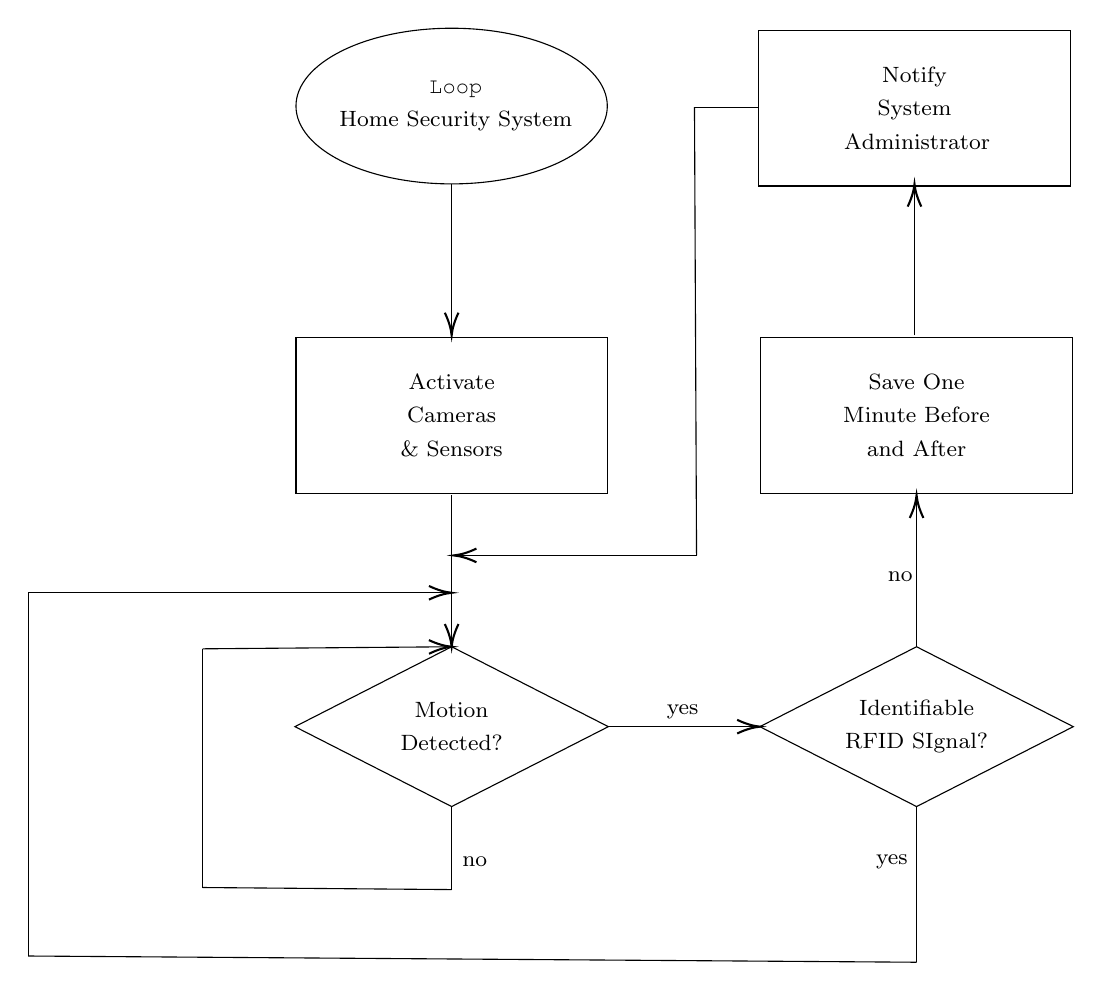
\begin{tikzpicture}[x=0.75pt,y=0.75pt,yscale=-1,xscale=1]
%uncomment if require: \path (0,469); %set diagram left start at 0, and has height of 469

%Shape: Ellipse [id:dp06026735517165571] 
\draw   (248,39.5) .. controls (248,18.79) and (281.58,2) .. (323,2) .. controls (364.42,2) and (398,18.79) .. (398,39.5) .. controls (398,60.21) and (364.42,77) .. (323,77) .. controls (281.58,77) and (248,60.21) .. (248,39.5) -- cycle ;
%Shape: Rectangle [id:dp880516595801381] 
\draw   (248,151) -- (398,151) -- (398,226) -- (248,226) -- cycle ;
%Straight Lines [id:da08375757950130125] 
\draw    (323,77) -- (323,148) ;
\draw [shift={(323,150)}, rotate = 270] [color={rgb, 255:red, 0; green, 0; blue, 0 }  ][line width=0.75]    (10.93,-3.29) .. controls (6.95,-1.4) and (3.31,-0.3) .. (0,0) .. controls (3.31,0.3) and (6.95,1.4) .. (10.93,3.29)   ;
%Flowchart: Decision [id:dp5735470816878454] 
\draw   (323,300) -- (398.5,338.5) -- (323,377) -- (247.5,338.5) -- cycle ;
%Straight Lines [id:da5891435380987948] 
\draw    (323,227) -- (323,298) ;
\draw [shift={(323,300)}, rotate = 270] [color={rgb, 255:red, 0; green, 0; blue, 0 }  ][line width=0.75]    (10.93,-3.29) .. controls (6.95,-1.4) and (3.31,-0.3) .. (0,0) .. controls (3.31,0.3) and (6.95,1.4) .. (10.93,3.29)   ;
%Shape: Boxed Line [id:dp9132377255103166] 
\draw    (398.5,338.5) -- (469.5,338.5) ;
\draw [shift={(471.5,338.5)}, rotate = 180] [color={rgb, 255:red, 0; green, 0; blue, 0 }  ][line width=0.75]    (10.93,-3.29) .. controls (6.95,-1.4) and (3.31,-0.3) .. (0,0) .. controls (3.31,0.3) and (6.95,1.4) .. (10.93,3.29)   ;
%Shape: Rectangle [id:dp6249646563980265] 
\draw   (472,151) -- (622,151) -- (622,226) -- (472,226) -- cycle ;
%Flowchart: Decision [id:dp8409280085137256] 
\draw   (547,300) -- (622.5,338.5) -- (547,377) -- (471.5,338.5) -- cycle ;
%Shape: Boxed Line [id:dp5338753000763605] 
\draw    (547,300) -- (547,229) ;
\draw [shift={(547,227)}, rotate = 90] [color={rgb, 255:red, 0; green, 0; blue, 0 }  ][line width=0.75]    (10.93,-3.29) .. controls (6.95,-1.4) and (3.31,-0.3) .. (0,0) .. controls (3.31,0.3) and (6.95,1.4) .. (10.93,3.29)   ;
%Straight Lines [id:da26354690571623807] 
\draw    (547,377) -- (547,452) ;
%Straight Lines [id:da7739477994676851] 
\draw    (119,449) -- (547,452) ;
%Straight Lines [id:da7947037860822463] 
\draw    (119,274) -- (119,449) ;
%Straight Lines [id:da7385058765120314] 
\draw    (119,274) -- (321,274) ;
\draw [shift={(323,274)}, rotate = 180] [color={rgb, 255:red, 0; green, 0; blue, 0 }  ][line width=0.75]    (10.93,-3.29) .. controls (6.95,-1.4) and (3.31,-0.3) .. (0,0) .. controls (3.31,0.3) and (6.95,1.4) .. (10.93,3.29)   ;
%Straight Lines [id:da8520509248377834] 
\draw    (323,377) -- (323,417) ;
%Straight Lines [id:da69771227917011] 
\draw    (203,416) -- (323,417) ;
%Straight Lines [id:da3020830480387937] 
\draw    (203,301) -- (203,416) ;
%Straight Lines [id:da6539681796101906] 
\draw    (203,301) -- (321,300.02) ;
\draw [shift={(323,300)}, rotate = 179.52] [color={rgb, 255:red, 0; green, 0; blue, 0 }  ][line width=0.75]    (10.93,-3.29) .. controls (6.95,-1.4) and (3.31,-0.3) .. (0,0) .. controls (3.31,0.3) and (6.95,1.4) .. (10.93,3.29)   ;
%Shape: Boxed Line [id:dp4681291110725898] 
\draw    (546,150) -- (546,79) ;
\draw [shift={(546,77)}, rotate = 90] [color={rgb, 255:red, 0; green, 0; blue, 0 }  ][line width=0.75]    (10.93,-3.29) .. controls (6.95,-1.4) and (3.31,-0.3) .. (0,0) .. controls (3.31,0.3) and (6.95,1.4) .. (10.93,3.29)   ;
%Shape: Rectangle [id:dp35495318125677144] 
\draw   (471,3) -- (621,3) -- (621,78) -- (471,78) -- cycle ;
%Straight Lines [id:da33391750072816073] 
\draw    (441,256) -- (326,256) ;
\draw [shift={(324,256)}, rotate = 360] [color={rgb, 255:red, 0; green, 0; blue, 0 }  ][line width=0.75]    (10.93,-3.29) .. controls (6.95,-1.4) and (3.31,-0.3) .. (0,0) .. controls (3.31,0.3) and (6.95,1.4) .. (10.93,3.29)   ;
%Straight Lines [id:da4629225097810108] 
\draw    (471,40) -- (440,40) ;
%Straight Lines [id:da9308190728302066] 
\draw    (440,40) -- (441,256) ;

% Text Node
\draw (325,39.5) node   [align=left] {\begin{minipage}[lt]{85.71pt}\setlength\topsep{0pt}
\begin{center}
{\fontfamily{pcr}\selectfont {\footnotesize Loop}}\\{\footnotesize Home Security System}
\end{center}

\end{minipage}};
% Text Node
\draw (323,188.5) node   [align=left] {\begin{minipage}[lt]{40.36pt}\setlength\topsep{0pt}
\begin{center}
{\footnotesize Activate}\\{\footnotesize Cameras}\\{\footnotesize \& Sensors}
\end{center}

\end{minipage}};
% Text Node
\draw (323,338.5) node   [align=left] {\begin{minipage}[lt]{39.92pt}\setlength\topsep{0pt}
\begin{center}
{\footnotesize Motion }\\{\footnotesize Detected?}
\end{center}

\end{minipage}};
% Text Node
\draw (434.34,336) node [anchor=south] [inner sep=0.75pt]   [align=left] {{\footnotesize yes}};
% Text Node
\draw (547,188.5) node   [align=left] {\begin{minipage}[lt]{53.53pt}\setlength\topsep{0pt}
\begin{center}
{\footnotesize Save One}\\{\footnotesize Minute Before}\\{\footnotesize  and After}
\end{center}

\end{minipage}};
% Text Node
\draw (547,338.5) node   [align=left] {\begin{minipage}[lt]{51.7pt}\setlength\topsep{0pt}
\begin{center}
{\footnotesize Identifiable}\\{\footnotesize RFID SIgnal?}
\end{center}

\end{minipage}};
% Text Node
\draw (546.36,266.5) node [anchor=east] [inner sep=0.75pt]   [align=left] {{\footnotesize no}};
% Text Node
\draw (546.69,403.5) node [anchor=east] [inner sep=0.75pt]   [align=left] {\begin{minipage}[lt]{15.43pt}\setlength\topsep{0pt}
\begin{center}
{\footnotesize yes}
\end{center}

\end{minipage}};
% Text Node
\draw (325,400) node [anchor=north west][inner sep=0.75pt]   [align=left] {\begin{minipage}[lt]{11.8pt}\setlength\topsep{0pt}
\begin{center}
{\footnotesize no}
\end{center}

\end{minipage}};
% Text Node
\draw (546,40.5) node   [align=left] {\begin{minipage}[lt]{50.79pt}\setlength\topsep{0pt}
\begin{center}
{\footnotesize Notify}\\{\footnotesize System}\\{\footnotesize Administrator}
\end{center}

\end{minipage}};


\end{tikzpicture}

  \caption{Home Security System Flowchart}
  \label{fig:1}
\end{figure}

\end{document}
